\section{DMA (Direct Memory Access)}\label{par:DMA}
Il \textbf{DMA} è un dispositivo che permette di sollevare il processore dall'onere di trasferire i dati tra varie periferiche. In particolare, il DMA permette di gestire il trasferimento dati tra:
\begin{itemize}
    \item \textbf{Memoria $\leftrightarrow$ Periferica};
    \item \textbf{Periferica $\leftrightarrow$ Memoria}
    \item \textbf{Memoria $\leftrightarrow$ Memroia}
\end{itemize}

Il suo principio di funzionamento è semplice, ed è schematizzabile su 3 registri principali:
\begin{itemize}
    \item \textbf{Registro Indirizzo}: Indica l'indirizzo da cui prelevare il dato;
    \item \textbf{Registro Conteggio}: Indica il conteggio del numero di "dati" trasferiti, e permette di capire quando bisogna interrompere il trasferimento;
    \item \textbf{Registro Identificativo}: Tramite tale registro si vanno ad identificare:
    \begin{itemize}
        \item o il dispositivo da considerare per il trasferimento;
        \item o l'area di memoria da considerare per il trasferimento.
    \end{itemize}  

\end{itemize}

La reale architettura del DMA è però più complessa. La maggior complessità dell'architettura proviene da varie tipologie di problematiche che si possono riscontrare durante il funzionamento, come, ad esempio, l'accesso al BUS dati in maniera concorrente al processore. \uppercase{è} pertanto necessario che il DMA non sia collegato al processore solo tramite il bus dato, ma anche tramite vari bus di controllo, che permettono al processore ed al DMA di poter comunicare e coordinarsi.

Il dispositivo a cui si fa riferimento nelle esercitazioni del corso è l'\textbf{Intel 8237}, che per la sua architettura ha 4 canali distinti (quindi è in grado di gestire 4 trasferimenti alla volta). Nella sua versione simulata in ASIM, tale componente è composto di soli 2 canali.
Scendendo più nei dettagli, il dispositivo reale è in grado di sostenere 4 modalità di funzionamento differenti, ovvero:
\begin{itemize}
    \item \textbf{Single}: Si trasferisce una \textit{word} alla volta; dopo aver trasferito una word, il DMA restituisce il BUS al processore almeno per un ciclo;
    \item \textbf{Block}: Si trasferisce un intero \textit{blocco} non appena il DMA acquisisce il BUS. Alla fine del trasferimento, viene inoltrata un'interruzione al processore che segnala la fine del trasferimento (e quindi la disponibilità del BUS);
    \item \textbf{On Demand}: Simile alla modalità Block, con l'unica differenza che il trasferimento può essere interrotto dal processore, per poi essere ripreso, grazie ai registri contatore, dall'esatto punto in cui era stato interrotto;
    \item \textbf{Cascade}: Modalità di funzionamento che permette di collegare più DMA in cascata in modo da poter gestire più di 4 canali.
\end{itemize}

Oltre al minor numero di canali, il componente simulato in ASIM non supporta tutte le modalità sopra-citate, difatti le modalità utilizzabili in ASIM sono \textbf{Single} e \textbf{Block}.\\
Guardando la figura [\ref{img:DMA}], abbiamo il modello architetturale del componente realizzato in ASIM, di cui i registri posti sulla sinistra sono di comunicazione con il processore, mentre i segnali sulla destra sono quelli che vengono utilizzati per l'interfacciamento con le periferiche collegate ai corrispettivi canali.

Per la comunicazione con il processore, il significato che hanno i segnali rappresentati è il seguente:
\begin{itemize}
    \item \textbf{D0-D7}: collegamento al BUS dati da e verso il componente;
    \item $\overline{\mathbf{CS}}$: segnale binario di selezione del dispositivo
    \item \textbf{A0-A3}: Attenzione! - non tutti i segnali Ai, ma solo i 4 meno significativi, vengono utilizzati per la selezione dello specifico registro interno da considerare;
    \item $\overline{\mathbf{IOR}}$ e $\overline{\mathbf{IOW}}$: Segnali di gestione della lettura e della scrittura sul componente e per le periferiche;
    \item $\overline{\mathbf{MEMR}}$ e $\overline{\mathbf{MEMW}}$: Segnali di gestione della lettura e della scrittura sui dispositivi di memoria;
    \item \textbf{CLK e Reset}: Classici segnali di clock (tempificazione delle operazioni) e reset (dei registri del dispositivo);
    \item \textbf{HRQ}: Segnale di richiesta del controllo del sistema BUS, che solitamente è collegata all'ingresso HOLD della CPU;
    \item \textbf{HLDA}: Segnale proveniente dalla CPU che segnala l'acquisizione del sistema BUS da parte del processore;
    \item  $\overline{\mathbf{EOP}}$: Linea di interruzione \textit{bidirezionale} che bisogna collegare al processore per segnalare il completamento del trasferimento richiesto.
\end{itemize}

Dati i due differenti canali si avranno 2 periferiche collegate allo stesso dispositivo DMA. Pertanto, la comunicazione, potrà essere effetuata da una sola di queste periferiche per volta. Tale decisione viene effettuata secondo un ordine di priorità, per cui il dispositivo collegato ai terminali 0 avrà una priorità maggiore rispetto a quello collegato ai terminali 1. I segnali che gestiscono le periferiche sono:
\begin{itemize}
    \item \textbf{DREQ0 e DREQ1}: Che sono due segnali che utilizzano le periferiche per richiedere l'accesso al BUS tramite dei cicli DMA;
    \item \textbf{DACK0 e DACK1}; Sono due segnali che permettono di comunicare alla periferica (da parte del DMA) la disponibilità a soddisfare una richiesta di accesso tramite DMA al bus.
\end{itemize}

\begin{figure}
    \centering
    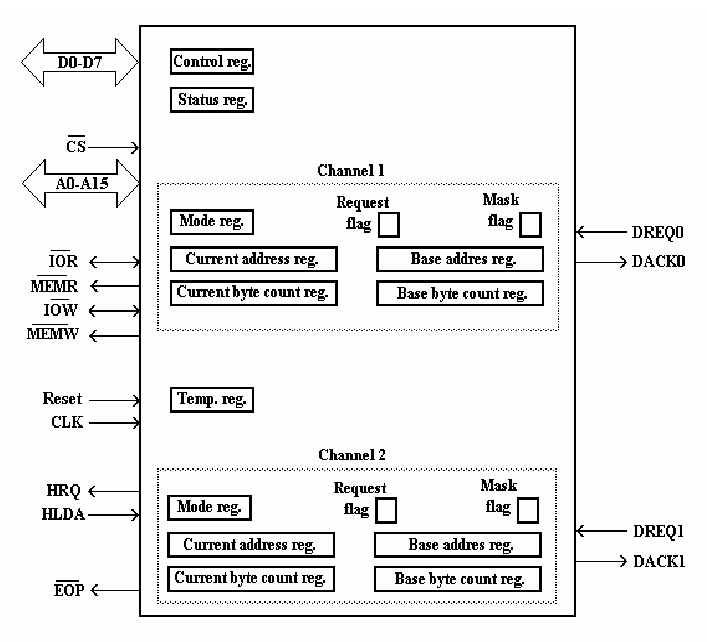
\includegraphics[width=.7\textwidth]{img/DMA.png}
    \caption{Modello di programmazione DMA a 2 canali}\label{img:DMA}
\end{figure}

\subsection{Utilizzo effettivo in ASIM}
Per capire al meglio come utilizzare il DMA, bisogna, in una prima fase, capire cosa tale DMA dovrà fare ed in che modo esso dovrà lavorare. Per definire queste cose vi sono i registri di controllo (unico per tutti i canali) ed i registri di Modo (uno per ogni canale). Quando si va a dischiarare il componente all'interno del file di configurazione, si vanno a definire due indirizzi (address 1 ed address 2), che permettano di scandire tra di loro sedici locazioni. Ciò ci serve per permetterci di poter accedere ai vari registri presenti all'interno del DMA, andandoli ad astrarre in registri di memoria (Memory-mapped). Precisamente, il funzionamento è gestito dal decodificatore collegato sul pin $\overline{\mathbf{CS}}$, che va ad attivare il pin quando rileva sul bus indirizzi un indirizzo appartenente all'insieme [address1, address2]. All'interno del file di configurazione vi sono anche le altre voci, che identificano specificatamente come il componente si collega ai vari BUS e ai vari componenti. Una buona architettura di tale sistema è quella che si può osservare nella figura [\ref{img:architettura-dma}]

\begin{figure}[h!]
    \centering
    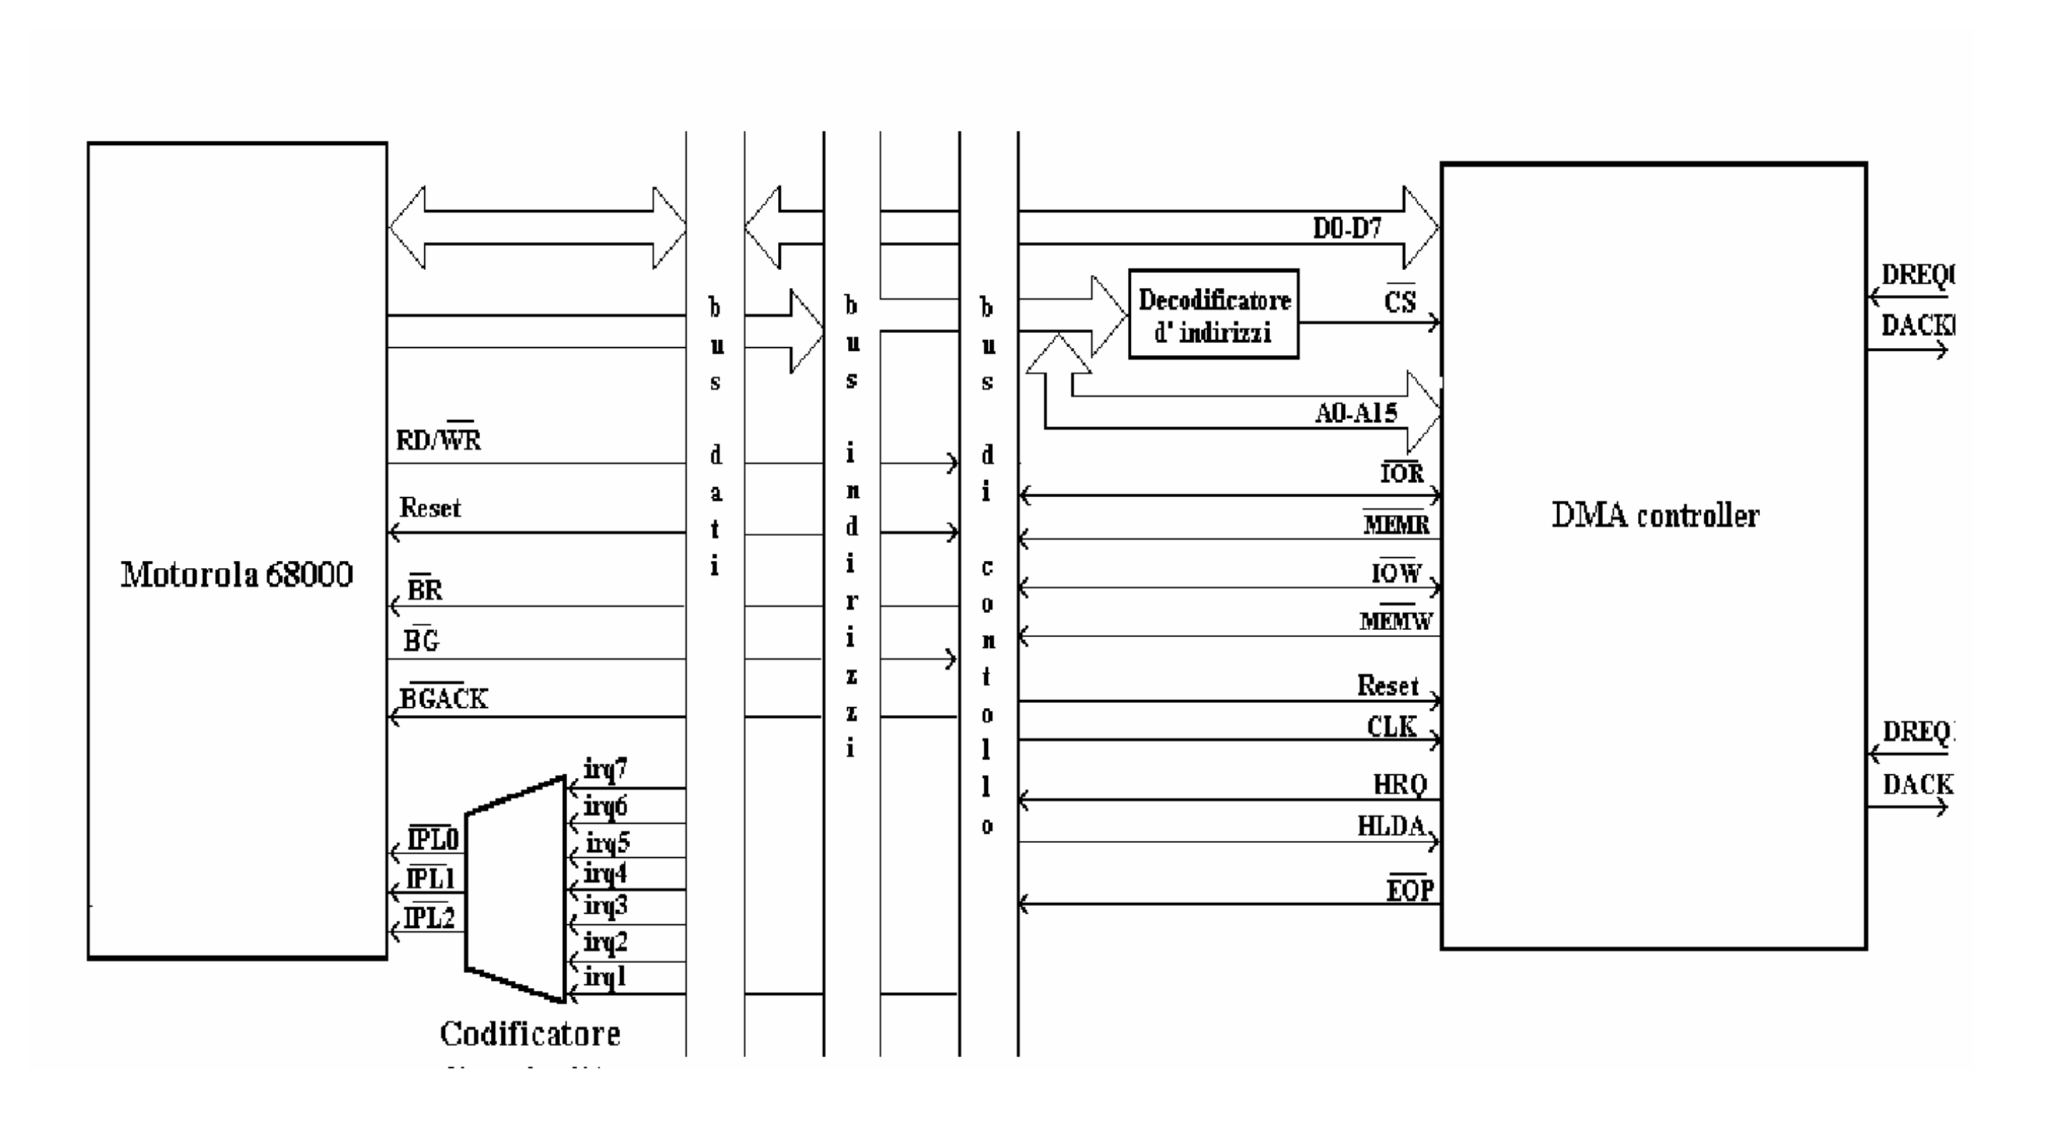
\includegraphics[width=.7\textwidth]{img/architettura-dma.png}
    \caption{Montaggio del componente DMA rispetto al sistema generale}\label{img:architettura-dma}
\end{figure}

Una volta compresa l'architettura del sistema, possiamo iniziare a comprendere in che modo andare a configurare il funzionamento del  DMA. Precisamente andiamo a vedere in primis il significato associato ai bit dei vari registri interni al componente.
Il primo registro che si può andare ad approfondire è il registro Mode, di cui ne sono presenti due, uno per ogni canale. Nella tabella \ref{tab:MODE-8237} sono illustrati i significati associati agli 8 bit del registro.

\begin{table}[h]
    \centering
    \begin{tabular}{|c|p{11cm}|}
    \hline
    \textbf{Bit} & \textbf{Significato} \\
    \hline
    0 & Instrada il dato su un canale, 0 per il canale 0 ed 1 per il canale 1 \\
    1-2 & Non utilizzati \\
    3 & Indica la direzione di trasferimento: 0 -> Da memoria ad interfaccia, 1 -> Da interfaccia a memoria \\
    4 & Abilita la \textbf{Autoinizializzazione}, e quindi se impostato a 1, quando il DMA termina il "conteggio" resetta i suoi registri con i reciproci registri di base \\
    5 & Definisce se vogliamo effettuare l'incremento di CADDR (caso di 0) oppure vogliamo impostare il decremento (caso di 1) \\
    6 & Non Utilizzato \\
    7 & Imposta la modalità di trasferimento: 0 -> Single, 1 -> Block. Ad ogni funzionamento si ha una gestione differente del BUS (nel caso block solo alla fine del trasferimento) \\
    \hline
    \end{tabular}
    \caption{Significato dei bit dei registri MODE}\label{tab:MODE-8237}
\end{table}

Oltre alla configurazione del singolo canale, devo anche impostare il registro di controllo dell'intero DMA controller.
\begin{table}[h]
    \centering
    \begin{tabular}{|c|p{11cm}|}
    \hline
    \textbf{Bit} & \textbf{Significato} \\
    \hline
    0 & Termina conteggio per il canale 0 \\
    1 & Termina conteggio per il canale 1 \\
    2 & è stata inoltrata una richiesta al canale 0 \\
    3 & è stata inoltrata una richiesta al canale 1 \\
    4 & Non Utilizzato \\
    5 & Abilita il trasferimento da memoria a memoria \\
    6 & Impone che in un trasferimento da memoria a memoria, l'indirizzo sorgente rimanga costante \\
    7 & Abilita il DMA controller \\
    \hline
    \end{tabular}
    \caption{Significato dei bit dei registri CTRL}\label{tab:CTRL-8237}
\end{table}

\subsection{Implementazione in Motorola 68k}
Le implementazioni in ASIM con motorola 68k sfruttano varie architetture (descritte dai file di configurazione). Una volta definita l'architettura si va a definire in che modo bisogna gestire i registri e l'iutilizzo delle periferiche (Come il DMA). Pertanto, bisogna distinguere i differenti utilizzi del DMA, per cui si divideranno le varie casistiche.

\subsubsection{Caso Memoria-Memoria}
Nel caso memoria-memoria, il DMA richiede una particolare definizione. Le prime cose che bisogna fare sono: definizione dell'area dati (dove prendere e dove trasferire i dati); definizione degli intervalli per l'accesso ai vari registri interni del DMA.
\begin{lstlisting}
* Area dati
                ORG 		$9500
origine	        DC.B		'0123456789 messaggio da trasferire'
destinazione	  DS.B	    34

* Definizione di indirizzo ed offset per l'accesso ai registri del DMA
dma		EQU 		$2010
caddr0		EQU		0
caddr1		EQU		2
ccount1	EQU		3
cntrl		EQU		8
mode		EQU		11
reset		EQU		13
clearmf	EQU		14
writeamf	EQU		15
nbyte		EQU		34
\end{lstlisting}

Una volta definita tutta la parte "statica" ovvero comprendente solo i dati utili per le configurazione, si passa alla parte operativa, dove si va a configurare effettivamente il dispositivo e si va ad avviare il suo funzionamento:
\begin{lstlisting}
        ORG 	$8200
        * Carico l'indirizzo del DMA
	    MOVE.W	    #dma,A0			

        * Carico l'indirizzo di origine dei dati all'interno del primo registro indirizzo
	    MOVE.W  	#origine,caddr0(A0)
        
        * Carico l'indirizzo di destinazione dei dati all'interno
        * del secondo registro indirizzo
        MOVE.W  	#destinazione,caddr1(A0)		

        * Carico il numero di caratteri da cui e' composta
        * la stringa all'interno del secondo counter
	    MOVE.B  	#nbyte,ccount1(A0)		

        * Imposto una comunicazione (in base ai bit) che 
        * dev'essere block, con incremento ed Autoinizializzazione
        * definendo una comunicazione memoria-interfaccia per il primo canale
        * Sto settando il primo canale utilizzando un VALORE pari
        MOVE.B  	#$90,mode(A0)		

        * Faccio una configurazione eguale a quella di prima solo che vario
        * il bit meno significativo per settare tramite VALORE
        * il secondo canale di comunicazione
	    MOVE.B	    #$91,mode(A0)		

        * Vado a settare l'ultimo registro, quello di controllo
        * che permette al DMA di poter iniziare a lavorare
	    MOVE.B	    #$A0,cntrl(A0)			

* Ciclo di attesa che simula lavoro del processore
loop	JMP	    loop
\end{lstlisting}

Una volta impostato il DMA e fatto partire, bisogna gestire l'interruzione che sarà scatenata quando esso avrà finito di lavorare. (pertanto, dato che stiamo lavorando con le interrupt, nel caso di asim, dobbiamo impostare la memoria in modo da inserire l'indirizzo della ISR all'interno della tabella delle ISR autovettorizzate).
L'ISR che si va a scrivere per il DMA, è una ISR che ha come unico scopo quello di resettare il DMA. Per cui si avrà:
\begin{lstlisting}
	    ORG $8700
int7	MOVE.L	A0,-(A7) *Salva il contesto
		MOVE.W	#dma,A0					
		MOVE.B	#0,reset(A0) *Resetta il DMA
		MOVE.L	(A7)+,A0 *Ripristina i registri utilizzati
		RTE
\end{lstlisting}
